\chapter{Linked Data}
As mentioned in the \nameref{sec:intro}, the evolution from \ac{bim} to \ac{ldbim} represents an evolution of the data \textbf{management} layer. This layer utilizes \emph{Linked Data} which, as stated by the \ac{w3c}, is a collection of interrelated datasets on the Web, formatted in a standard way that is accessible and manageable by Semantic Web tools. The same applies to the relationships among them.\footcite{w3c} The following collection of Semantic Web technologies explores the required environment to achieve this goal.

\section{\acs{rdf} and triples} \label{subsec:rdfAndTriples}
At the core of the Semantic Web is the \ac{rdf}, a data model for describing resources on the Web. RDF is a graph data model that consists of \textbf{triples}, which are statements about resources. A triple consists of a subject, a predicate, and an object. The subject is the resource that is being described, the predicate is the property of the subject, and the object is the value of the property. Both the predicate and the object can, in turn, become the subjects of other triples. Listing \ref{lst:rdfSample} shows an example of an \ac{rdf} database described in the Turtle format.

\begin{figure}[H]
    \centering
    

\tikzset{every picture/.style={line width=0.75pt}} %set default line width to 0.75pt        

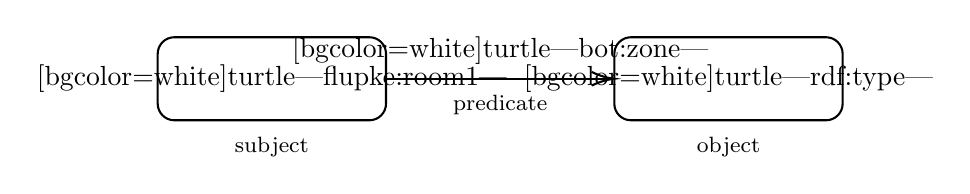
\begin{tikzpicture}[x=0.75pt,y=0.75pt,yscale=-1,xscale=1]
    %uncomment if require: \path (0,300); %set diagram left start at 0, and has height of 300

    %Rounded Rect [id:dp16428191799546488] 
    \draw   (80,68) .. controls (80,63.58) and (83.58,60) .. (88,60) -- (182,60) .. controls (186.42,60) and (190,63.58) .. (190,68) -- (190,92) .. controls (190,96.42) and (186.42,100) .. (182,100) -- (88,100) .. controls (83.58,100) and (80,96.42) .. (80,92) -- cycle ;
    %Rounded Rect [id:dp211253547738401] 
    \draw   (300,68) .. controls (300,63.58) and (303.58,60) .. (308,60) -- (402,60) .. controls (406.42,60) and (410,63.58) .. (410,68) -- (410,92) .. controls (410,96.42) and (406.42,100) .. (402,100) -- (308,100) .. controls (303.58,100) and (300,96.42) .. (300,92) -- cycle ;
    %Straight Lines [id:da3976910390317223] 
    \draw    (190,80) -- (298,80) ;
    \draw [shift={(300,80)}, rotate = 180] [color={rgb, 255:red, 0; green, 0; blue, 0 }  ][line width=0.75]    (10.93,-3.29) .. controls (6.95,-1.4) and (3.31,-0.3) .. (0,0) .. controls (3.31,0.3) and (6.95,1.4) .. (10.93,3.29)   ;

    % Text Node
    \draw (135,80) node   [align=left] {\mintinline[bgcolor=white]{turtle}|flupke:room1|};
    % Text Node
    \draw (355,80) node   [align=left] {\mintinline[bgcolor=white]{turtle}|rdf:type|};
    % Text Node
    \draw (245,66.5) node   [align=left] {\mintinline[bgcolor=white]{turtle}|bot:zone|};
    % Text Node
    \draw (135,113) node  [font=\footnotesize] [align=left] {subject};
    % Text Node
    \draw (355,113) node  [font=\footnotesize] [align=left] {object};
    % Text Node
    \draw (245,92.5) node  [font=\footnotesize] [align=left] {predicate};


\end{tikzpicture}

    \caption{Triple structure}
    \label{fig:triple}
\end{figure}

The basic, yet versatile, structure of a triple is illustrated in Figure \ref{fig:triple}. Both the subject and object are considered as nodes in the data graph, and they are linked by the predicate, which is referred to as an edge. Multiple triples can thus create and link multiple nodes or enrich a connection between two nodes by creating new edges between them. Each element contains a single resource that can be one of the three types: a \acs{uri}, a literal, or a blank node. A \ac{uri} identifies the name and/or location of a resource on the web and, as its name states, is unique and unambiguous, thus enabling queries and reasoning of the same nature. A literal is a value, and a blank node is an anonymous resource, sometimes used as a placeholder when the exact resource is not known or not necessary to specify. Due to their nature, a subject must be either a \ac{uri} or a blank node, a predicate exclusively a \ac{uri}, and the object may be any of the three types. As \ac{uri} descriptions can be very long, a prefix can be used to shorten them. This is illustrated in Listing \ref{lst:rdfSample} with the \mintinline{turtle}|@prefix bot: <https://w3id.org/bot#>|, which declares that \mintinline{turtle}|bot:Zone| refers, in its full length, to the address \mintinline{turtle}|<https://w3id.org/bot#Zone>|.

\begin{listing}[H]
    \inputminted{turtle}{figures/snippets/rdfSample.ttl}
    \vspace{-0.7cm}
    \caption{Example of an \acs{rdf} database in turtle format}
    \label{lst:rdfSample}
\end{listing}

This basic concept can be extrapolated to describe and store any kind of data. The advantage for the \ac{aec} industry would be to allow any stakeholders to describe and enrich the knowledge base of a building.

\section{Ontologies and reasoning}\label{subsec:ontologies}
When looking at Listing \ref{lst:rdfSample}, a distinction can be made between two types of statements: some refer to classes or properties, such as \mintinline{turtle}|bot:Zone| or \mintinline{turtle}|bot:containsElement|, while others refer to instances such as \mintinline{turtle}|flupke:room1|. The former is referred to as the TBox for \enquote{terminology}, and the latter is referred to as the ABox for \enquote{assertions}. The TBox, the ontology layer, is used to describe instances in the ABox and their relationships.

By developing an ontology, the domain of interest and the relationships between the classes and properties can be described. This is achieved by defining the classes and properties of the domain and their relationships. The ontology is then used to reason about the domain, inferring new facts based on the ontology and the existing facts within the domain. This is done by a reasoner, which is software capable of performing the reasoning itself on the ontology and associated data. As mentioned, the reasoner can be used to infer new facts, check if created facts are consistent with the ontology, and check if the ontology itself is consistent.\footcite{w3cInfering} It is often integrated with \ac{rdf} databases, also known as triplestores or graph databases.

Classes, properties, and their relationships can be defined using \ac{rdfs}, which is a vocabulary for describing \ac{rdf} schemas using a basic set of constructs. As an extension of \ac{rdfs}, \ac{owl} is a vocabulary for describing ontologies using a more expressive set of constructs tailored to the needs of ontologies. Both \ac{rdfs} and \ac{owl} are considered to be formal ontologies themselves, as they describe the classes and properties of the domain of \ac{rdf}.

\section{Triplestores and \acs{sparql}}
As briefly discussed in \ref{subsec:ontologies}, triplestores are \ac{rdf} databases that store data in the form of a graph. They are used to store and query Linked Data and are often integrated with a reasoner. The data itself is retrieved and modified using the \ac{sparql}.\footcite{w3cQuery} In contrast to \ac{sql}, \ac{sparql} queries are able to work across multiple triplestores, called \ac{sparql} endpoints. These are known as federated queries, and their results are combined into a single result set. This is useful when the data is distributed across multiple triplestores in a decentralized manner.\footcite{ontotextSpaql} For example, multiple stakeholders participating in a project, each with their own database.

\section{Complexity of the data graph}
The complexity of the data graph is a major concern when working with \ac{ldbim}. This section discusses the origins of the different sources of geometric data that enrich it. Firstly, by looking at the different \ac{lod}'s that can be used to describe a building, which already exists in the \ac{bim} domain. Secondly, by looking at \ac{ldbim} and the exponential growth it imposes on the data graph.

\begin{figure}[H]
    \centering
    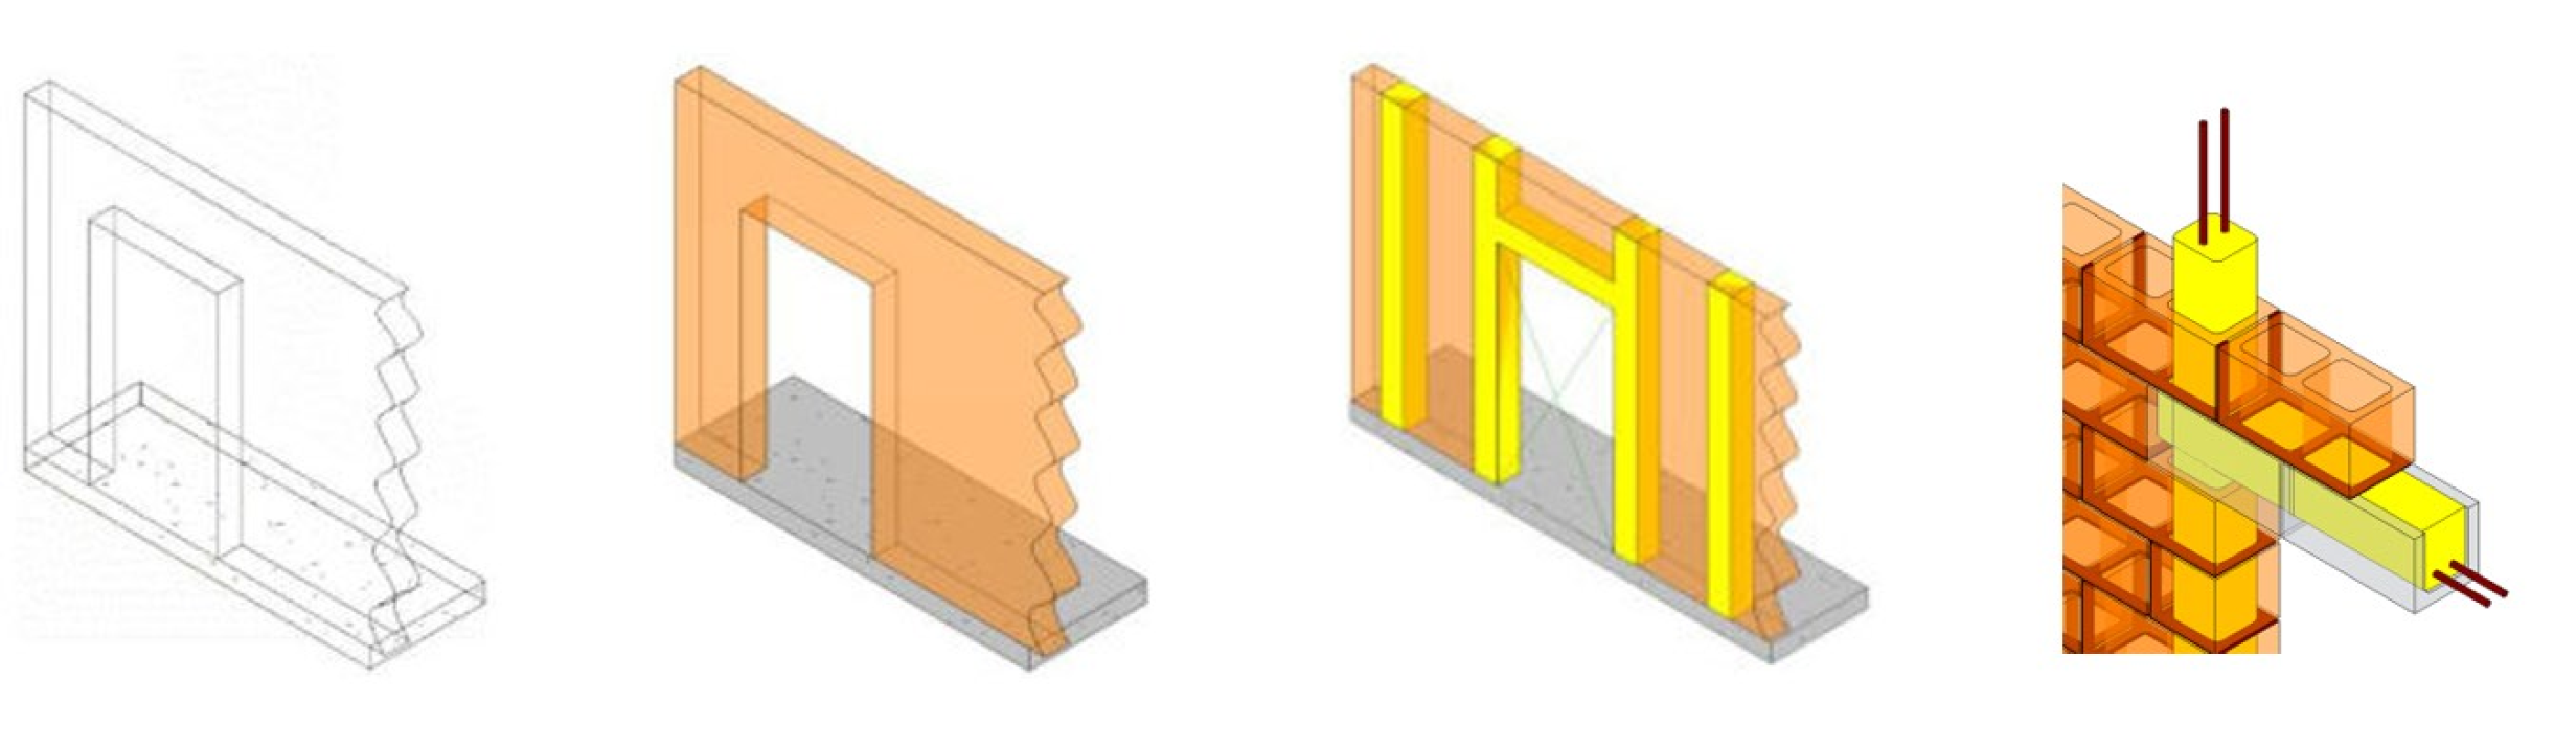
\includegraphics[width=\textwidth]{figures/pdf/LOD.pdf}
    \caption[\acs{lod} evolution]{\acs{lod} evolution\\ from \cite{lod}}
    \label{fig:LOD}
\end{figure}

\subsection{\acs{bim} geometry} \label{subsec:bimGeometry}
The 3D model of a building consists of a multitude of sub-models, describing objects for all the different stakeholders participating in the project. Some describe very large objects, and some very small parts. Both can be defined in their most simple and abstract form or have an intricate and complex geometry. For instance, a door can simply be defined as a box, or up to the level of the screw-thread for the hinge system. The level of abstraction is here described as the \ac{lod}, which is most of the time pre-selected for the needs of a \ac{bim} model, and is applied throughout a single model.

As shown in Figure~\ref{fig:LOD}, a standard BIM workflow goes through multiple phases, each with their associated model and \ac{lod}. This makes it an important concept in the \ac{aec} industry, as it allows for a very efficient workflow. The modeling step is approached from a top-down perspective, starting with rougher geometries describing the broader ideas of a concept model and evolving to a more refined model for the construction documentation phase. As the last and longest-standing model, a higher \ac{lod} can be used to describe subtle changes in the evolution of a building during the operation phase.

\subsection{\acs{ldbim} geometry}
The interconnectivity of semantics can also be applied to geometry descriptions. This could allow the co-existence of multiple \ac{lod}s in a single model database. Besides storing the evolution of a single element's geometry, it enables the linking of the different \ac{lod}s, described in \ref{subsec:bimGeometry}, to each other. Not only that, but extending onto the size of the models described in Table \ref{tab:sizeModels}, already existing \ac{mep}, structural, alongside many other stakeholders' geometry can be added.